%% Lab Report for EEET2493_labreport_template.tex
%% V1.0
%% 2019/01/16
%% This is the template for a Lab report following an IEEE paper. Modified by Francisco Tovar after Michael Sheel original document.


%% This is a skeleton file demonstrating the use of IEEEtran.cls
%% (requires IEEEtran.cls version 1.8b or later) with an IEEE
%% journal paper.
%%
%% Support sites:
%% http://www.michaelshell.org/tex/ieeetran/
%% http://www.ctan.org/pkg/ieeetran
%% and
%% http://www.ieee.org/

%%*************************************************************************
%% Legal Notice:
%% This code is offered as-is without any warranty either expressed or
%% implied; without even the implied warranty of MERCHANTABILITY or
%% FITNESS FOR A PARTICULAR PURPOSE! 
%% User assumes all risk.
%% In no event shall the IEEE or any contributor to this code be liable for
%% any damages or losses, including, but not limited to, incidental,
%% consequential, or any other damages, resulting from the use or misuse
%% of any information contained here.
%%
%% All comments are the opinions of their respective authors and are not
%% necessarily endorsed by the IEEE.
%%
%% This work is distributed under the LaTeX Project Public License (LPPL)
%% ( http://www.latex-project.org/ ) version 1.3, and may be freely used,
%% distributed and modified. A copy of the LPPL, version 1.3, is included
%% in the base LaTeX documentation of all distributions of LaTeX released
%% 2003/12/01 or later.
%% Retain all contribution notices and credits.
%% ** Modified files should be clearly indicated as such, including  **
%% ** renaming them and changing author support contact information. **
%%*************************************************************************

\documentclass[journal]{IEEEtran}

% *** CITATION PACKAGES ***
\usepackage[style=ieee]{biblatex} 

% *** MATH PACKAGES ***
\usepackage{amsmath}

% *** PDF, URL AND HYPERLINK PACKAGES ***
\usepackage{url}
% correct bad hyphenation here
\hyphenation{op-tical net-works semi-conduc-tor}
\usepackage{graphicx}  %needed to include png, eps figures
\usepackage{float}  % used to fix location of images i.e.\begin{figure}[H]

%https://tex.stackexchange.com/questions/230828/when-referencing-a-figure-make-text-and-figure-name-clickable
\usepackage[colorlinks]{hyperref}

\usepackage{pdflscape}
\usepackage{multicol}
\usepackage{listings}
\usepackage{color}
\usepackage[dvipsnames]{xcolor}

%https://tex.stackexchange.com/questions/245842/i-am-trying-to-get-the-image-full-screen-and-landscape
\usepackage{graphicx}
\usepackage[a4paper,margin=1in]{geometry}
\usepackage{lscape}
\usepackage{rotating}
\usepackage{pdflscape}

\definecolor{dkgreen}{rgb}{0,0.6,0}
\definecolor{gray}{rgb}{0.5,0.5,0.5}
\definecolor{mauve}{rgb}{0.58,0,0.82}

\lstset{frame=tb,
language=C++,
aboveskip=3mm,
  belowskip=3mm,
  showstringspaces=false,
  columns=flexible,
  basicstyle={\small\ttfamily},
  numbers=none,
  numberstyle=\tiny\color{gray},
  keywordstyle=\color{blue},
  commentstyle=\color{dkgreen},
  stringstyle=\color{mauve},
  breaklines=true,
  breakatwhitespace=true,
  tabsize=3,
  %https://stackoverflow.com/questions/3915709/latex-lstlisting-automatically-recognizing-code-passage
  rangeprefix=//-LaTeX:,
  rangesuffix=;,
  includerangemarker=false,
  columns=spaceflexible,
  %https://tex.stackexchange.com/questions/106770/how-to-add-line-numbers-to-a-program-listing-code
  numbers=left,
  stepnumber=1
}

\lstdefinelanguage{Ini}
{
    basicstyle=\ttfamily\small,
    columns=fullflexible,
    morecomment=[s][\color{mauve}\bfseries]{[}{]},
    morecomment=[l]{\#},
    morecomment=[l]{;},
    commentstyle=\color{gray}\ttfamily,
    morekeywords={},
    otherkeywords={=,:},
    keywordstyle={\color{green}\bfseries}
}

% https://github.com/GothenburgBitFactory/guides/blob/master/20151107_de_openrheinruhr/yaml_syntax_highlighting.tex
%%%%%%%%%%%%%%%%%%%%%%%%%%%%%%%%%%%%%%%%%%%%%%%%%%%%%%
%%%%%%%%%%% YAML syntax highlighting %%%%%%%%%%%%%%%%%

% http://tex.stackexchange.com/questions/152829/how-can-i-highlight-yaml-code-in-a-pretty-way-with-listings

% here is a macro expanding to the name of the language
% (handy if you decide to change it further down the road)
\newcommand\YAMLcolonstyle{\color{red}\mdseries}
\newcommand\YAMLkeystyle{\color{black}\bfseries}
\newcommand\YAMLvaluestyle{\color{blue}\mdseries}

\makeatletter

\newcommand\language@yaml{yaml}

\expandafter\expandafter\expandafter\lstdefinelanguage
\expandafter{\language@yaml}
{
  keywords={true,false,null,y,n},
  keywordstyle=\color{darkgray}\bfseries,
  basicstyle=\YAMLkeystyle,                                 % assuming a key comes first
  sensitive=false,
  comment=[l]{\#},
  morecomment=[s]{/*}{*/},
  commentstyle=\color{purple}\ttfamily,
  stringstyle=\YAMLvaluestyle\ttfamily,
  moredelim=[l][\color{orange}]{\&},
  moredelim=[l][\color{magenta}]{*},
  moredelim=**[il][\YAMLcolonstyle{:}\YAMLvaluestyle]{:},   % switch to value style at :
  morestring=[b]',
  morestring=[b]",
  literate =    {---}{{\ProcessThreeDashes}}3
                {>}{{\textcolor{red}\textgreater}}1     
                {|}{{\textcolor{red}\textbar}}1 
                {\ -\ }{{\mdseries\ -\ }}3,
}

% switch to key style at EOL
\lst@AddToHook{EveryLine}{\ifx\lst@language\language@yaml\YAMLkeystyle\fi}
\makeatother

\newcommand\ProcessThreeDashes{\llap{\color{cyan}\mdseries-{-}-}}

%%%%%%%%%%% YAML syntax highlighting %%%%%%%%%%%%%%%%%
%%%%%%%%%%%%%%%%%%%%%%%%%%%%%%%%%%%%%%%%%%%%%%%%%%%%%%

\begin{document}

% paper title
\title{Arduino Lab 2}

% author names 
\author{Knut Ola Nøsen
}% <-this % stops a space

% The report headers
\markboth{IELET1002 DATATEKNIKK. LAB. REPORT 2, FEBRUARY 2022}%do not delete next lines
{Shell \MakeLowercase{\textit{et al.}}: Bare Demo of IEEEtran.cls for IEEE Journals}

% make the title area
\maketitle

% As a general rule, do not put math, special symbols or citations
% in the abstract or keywords.
\begin{abstract}
    The project explores how to control DC motors and servos. For the DC motor we are using the L293D chip, and for the servos we use the builtin Servo.h library.
    The reason for using the L293D chip is that motors not only require a lot more power than the Arduino can provide, but also more fine control than a relay.
    In this lab we will implement several ways of controlling motor speed, motor acceleration and servo position.
\end{abstract}

\begin{IEEEkeywords}
    Arduino, L293D, Servo, DC Motor, RAMP, PWM
\end{IEEEkeywords}

\section{Theory}
% Here we have the typical use of a "W" for an initial drop letter
% and "RITE" in caps to complete the first word.
% You must have at least 2 lines in the paragraph with the drop letter
% (should never be an issue)

\IEEEPARstart{W}{e}
start with the motor.
The L293D chip has two input pins (In1 and In2) for
specifying directions, and one input pin (Enable) for
setting speed with a PWM signal. The H-bridge derives its
name from the H-shaped design, with the vertical lines representing
a MOSFET, and the horizontal lines representing a motor.
The mosfets are enabled/disabled in diagonal pairs, in order to switch
the direction of the current. The directional MOSFETs are controlled by
2 transistors each. The transistors are connected inseries, where one
transistor enables/disables the mosfet, and the other forwars the PWM signal.
The following code shows how the L293D chip is used:
\begin{lstlisting}
   
void updateMotor(
    bool direction, 
    int speed, 
    int in1Pin, 
    int in2Pin, 
    int enablePin
)
{
    digitalWrite(
        in1Pin, 
        direction ? HIGH : LOW
    );
    digitalWrite(
        in2Pin, 
        direction ? LOW : HIGH
    );
    analogWrite(enablePin, speed);
}

\end{lstlisting}

While this code clearly displays how the L293D chip is used, it still lacks some safeguards that should be in
place on a DC-Motor. For example, brushed DC-Motors have a minimum voltage, before which they do not have
suficient power to start moving. We will implement this safeguard later.

\vfill\null
\pagebreak

\section{Methods}
\subsection{Hardware}

\begin{figure}[H]%[!ht]
    \begin {center}
    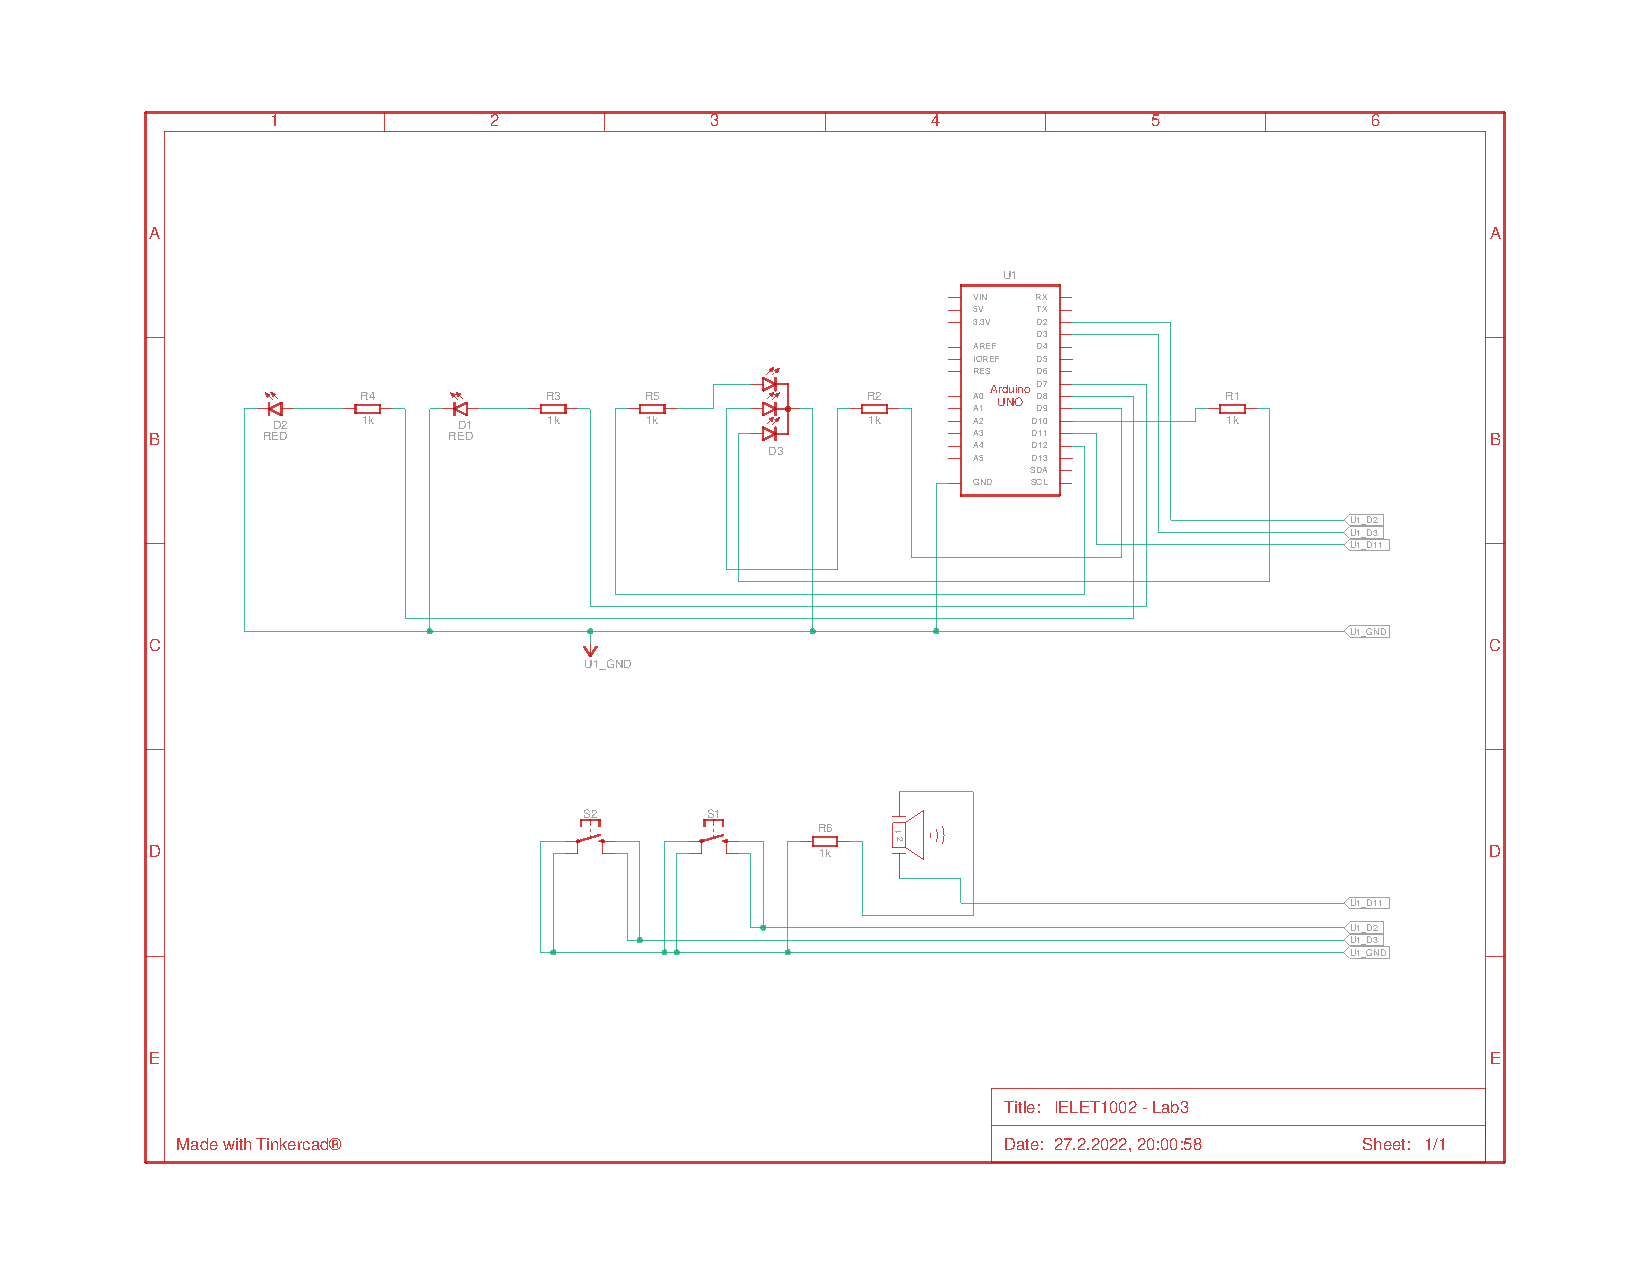
\includegraphics[width=0.45\textwidth, trim={0 2cm 0 2cm}]{images/wiring-diagram.pdf}
    \caption{Wiring Diagram}
    \label{fig:wiring}
    \end {center}
\end{figure}

\begin{figure}[H]%[!ht]
    \begin {center}
    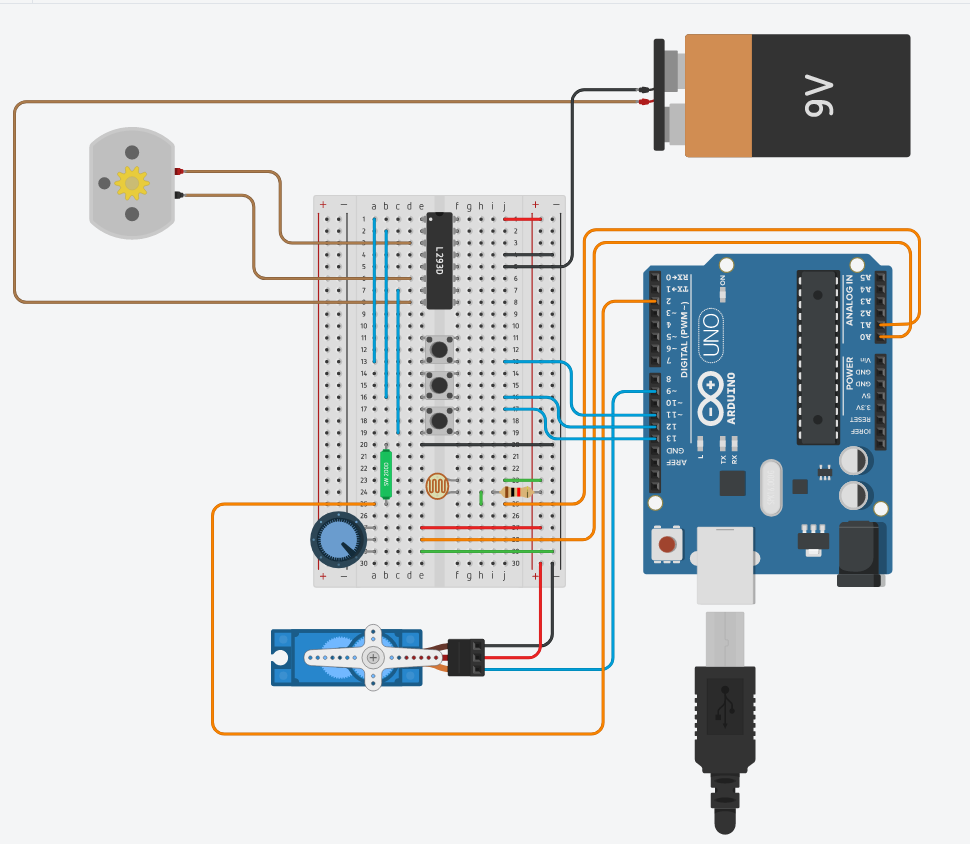
\includegraphics[width=0.45\textwidth]{images/tinkercad.PNG}
    \caption{Tinkercad}
    \label{fig:tinkercad}
    \end {center}
\end{figure}

\begin{figure}[H]
    \begin {center}
    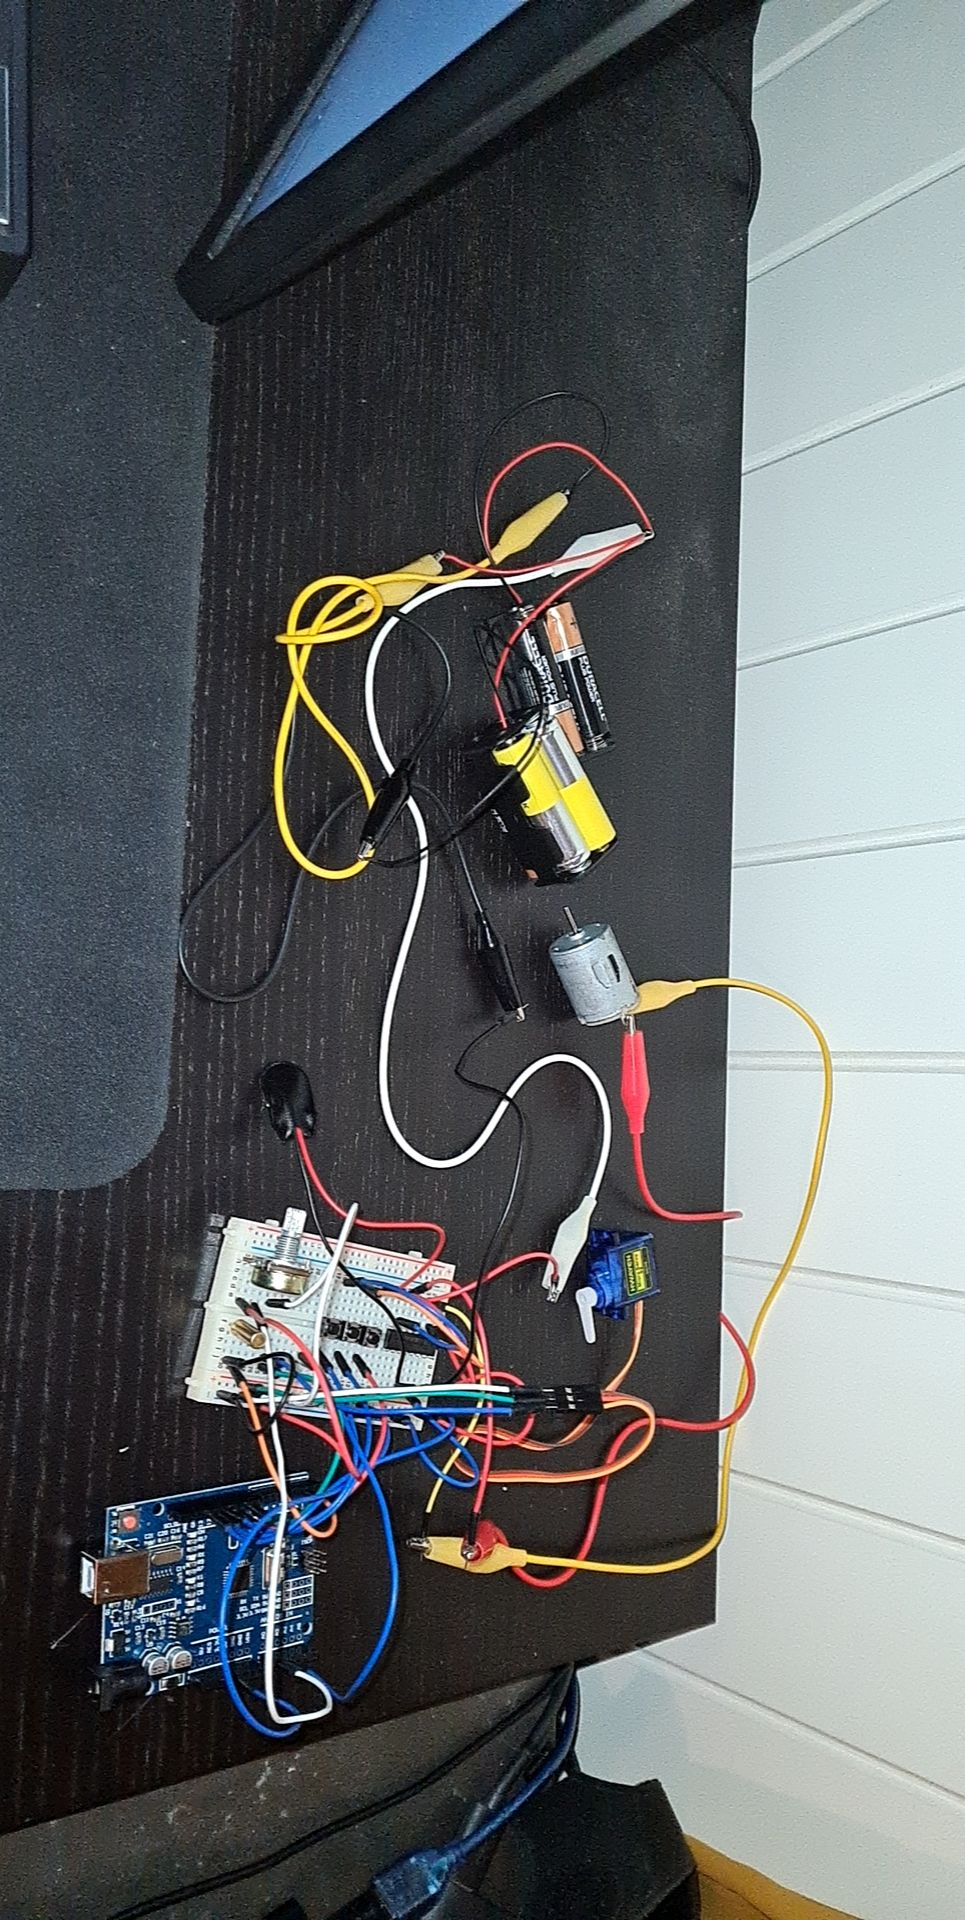
\includegraphics[width=0.25\textwidth, angle=90]{images/circuit-picture.jpg}
    \caption{Lab2 Circuit}
    \label{fig:circuitPicture}
    \end {center}
\end{figure}

\vfill\null
\pagebreak

\subsection{Software}
Lets start by creating some configs to keep our code free of "magic constants".
By keeping these configs in separate files, we avoid cluttering our logic in the main.cpp file.\\

\lstinputlisting[language=C++, caption=Range.h]{../lib/Range/Range.h}
\lstinputlisting[language=C++, caption=ServoConfig.h]{../lib/ServoConfig/ServoConfig.h}
\lstinputlisting[language=C++, caption=MotorConfig.h]{../lib/MotorConfig/MotorConfig.h}

\vfill\null
\pagebreak


\lstinputlisting[language=C++, caption=ApplicationConfig.h]{../lib/ApplicationConfig/ApplicationConfig.h}
This gives us a global const appConfig when we include the ApplicationConfig.h file
in our main sketch.

\vfill\null
\pagebreak

\onecolumn

We also define a class for the Photoresistor so we can get rid of those pesky globas.
\lstinputlisting[language=C++, caption=Photoresistor.h]{../lib/Photoresistor/Photoresistor.h}

\vfill\null
\pagebreak

Now that all our external files are set up, we can start looking at the main.cpp file.
%https://stackoverflow.com/questions/3915709/latex-lstlisting-automatically-recognizing-code-passage
\lstinputlisting[language=C++, caption=main.cpp - imports, linerange=imports-End_Section]{../src/main.cpp}

\lstinputlisting[language=C++, caption=main.cpp - CLAMPING           , linerange=CLAMPING-End_Section]{../src/main.cpp}
We add some clamping functions to restrict servo position and motor power to set ranges.
This way, we can avoid pushing our hardware beyone what it can do, without risking
human error while programming.

\lstinputlisting[language=C++, caption=main.cpp - Servo Control      , linerange=Servo_Control-End_Section]{../src/main.cpp}
Here we pipe our servo positioning through a guarded function that keeps us
within the hardware limits, similar to how we will with our DC motor.

\vfill\null
\pagebreak

\lstinputlisting[language=C++, caption=main.cpp - Motor Control      , linerange=Motor_Control-End_Section]{../src/main.cpp}
We create an enum for motor direction to be crystal clear about what is going on. We also add an overload
to setMotorSpeed that automatically sets direction based on a range that can accept negative speed.
This is useful for the centered potmeter controls, while it would pose problems during our ramp functions.

\vfill\null
\pagebreak

\lstinputlisting[language=C++, caption=main.cpp - Emergency Stop     , linerange=Emergency_Stop-End_Section]{../src/main.cpp}
For the emergency stop we continously keep killing the motors power by setting its direction to none.
This way, we are absolutely sure that nothing moves until the Emergency Stop is released.

\lstinputlisting[language=C++, caption=main.cpp - Setup              , linerange=setup-End_Section]{../src/main.cpp}

\lstinputlisting[language=C++, caption=main.cpp - Center Potmeter    , linerange=Center_Potmeter-End_Section]{../src/main.cpp}
In order to make our code more consise, we create a helper function for centering a potmeter reading.

\vfill\null
\pagebreak

\lstinputlisting[language=C++, caption=main.cpp - Exercise 3         , linerange=Exercise_3-End_Section]{../src/main.cpp}
Because the RAMP.h library can not (to my knowledge) handle negative ranges, we must handle this ourselves by explicitly
setting the direction, moving from 0 to 255, back to 0 and then to -255 etc.

\lstinputlisting[language=C++, caption=main.cpp - Exercise 4         , linerange=Exercise_4-End_Section]{../src/main.cpp}
Because we created some robust reusable code earlier, exercise 4 is now a lot easier.

\lstinputlisting[language=C++, caption=main.cpp - Exercise 6         , linerange=Exercise_6-End_Section]{../src/main.cpp}

\vfill\null
\pagebreak

\lstinputlisting[language=C++, caption=main.cpp - Exercise 7         , linerange=Exercise_7-End_Section]{../src/main.cpp}

\lstinputlisting[language=C++, caption=main.cpp - Exercise 8         , linerange=Exercise_8-End_Section]{../src/main.cpp}

\lstinputlisting[language=C++, caption=main.cpp - Exercise 9         , linerange=Exercise_9-End_Section]{../src/main.cpp}

\lstinputlisting[language=C++, caption=main.cpp - loop               , linerange=loop-End_Section]{../src/main.cpp}


\section{Discussion}
The current code works excellently, however it does have a weakness.
While the nested nature of this code makes for very few instances of "state" and
globals, it does prevent us from running continous updates on anything while
a piece of code is executing. In a larger project, i believe it would be
beneficial to avoid while and for-loops, in favour of a more flat architecture with
state machines. That way, the project remains scalable, and we can easily add
continous checks without risking spagheti code and human errors due to forgetting
to call an updater during a special loop.


\begin{landscape}

    \section{Large Images}

    \begin{figure}[h]
        \begin {center}
        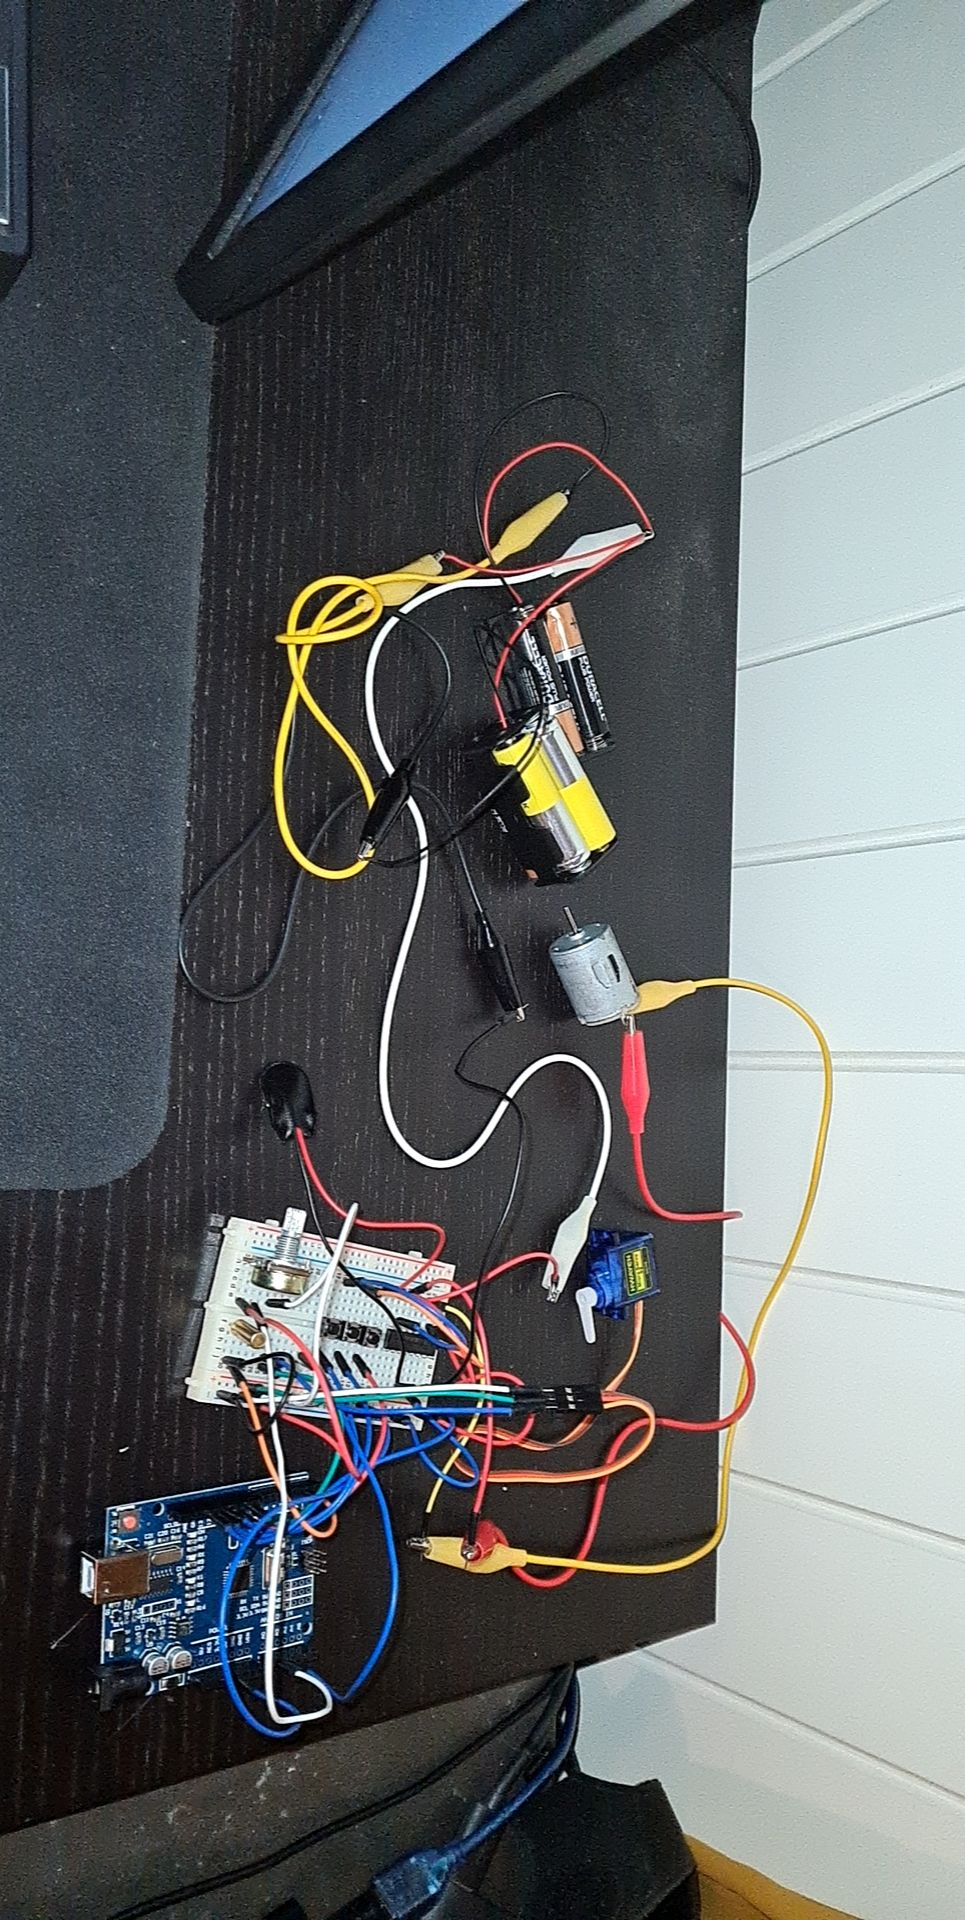
\includegraphics[width=0.8\textwidth, angle=90]{images/circuit-picture.jpg}
        \caption{Large Lab2 Circuit}
        \label{fig:circuitPictureLarge}
        \end {center}
    \end{figure}

    \begin{figure}[h]%[!ht]
        \begin {center}
        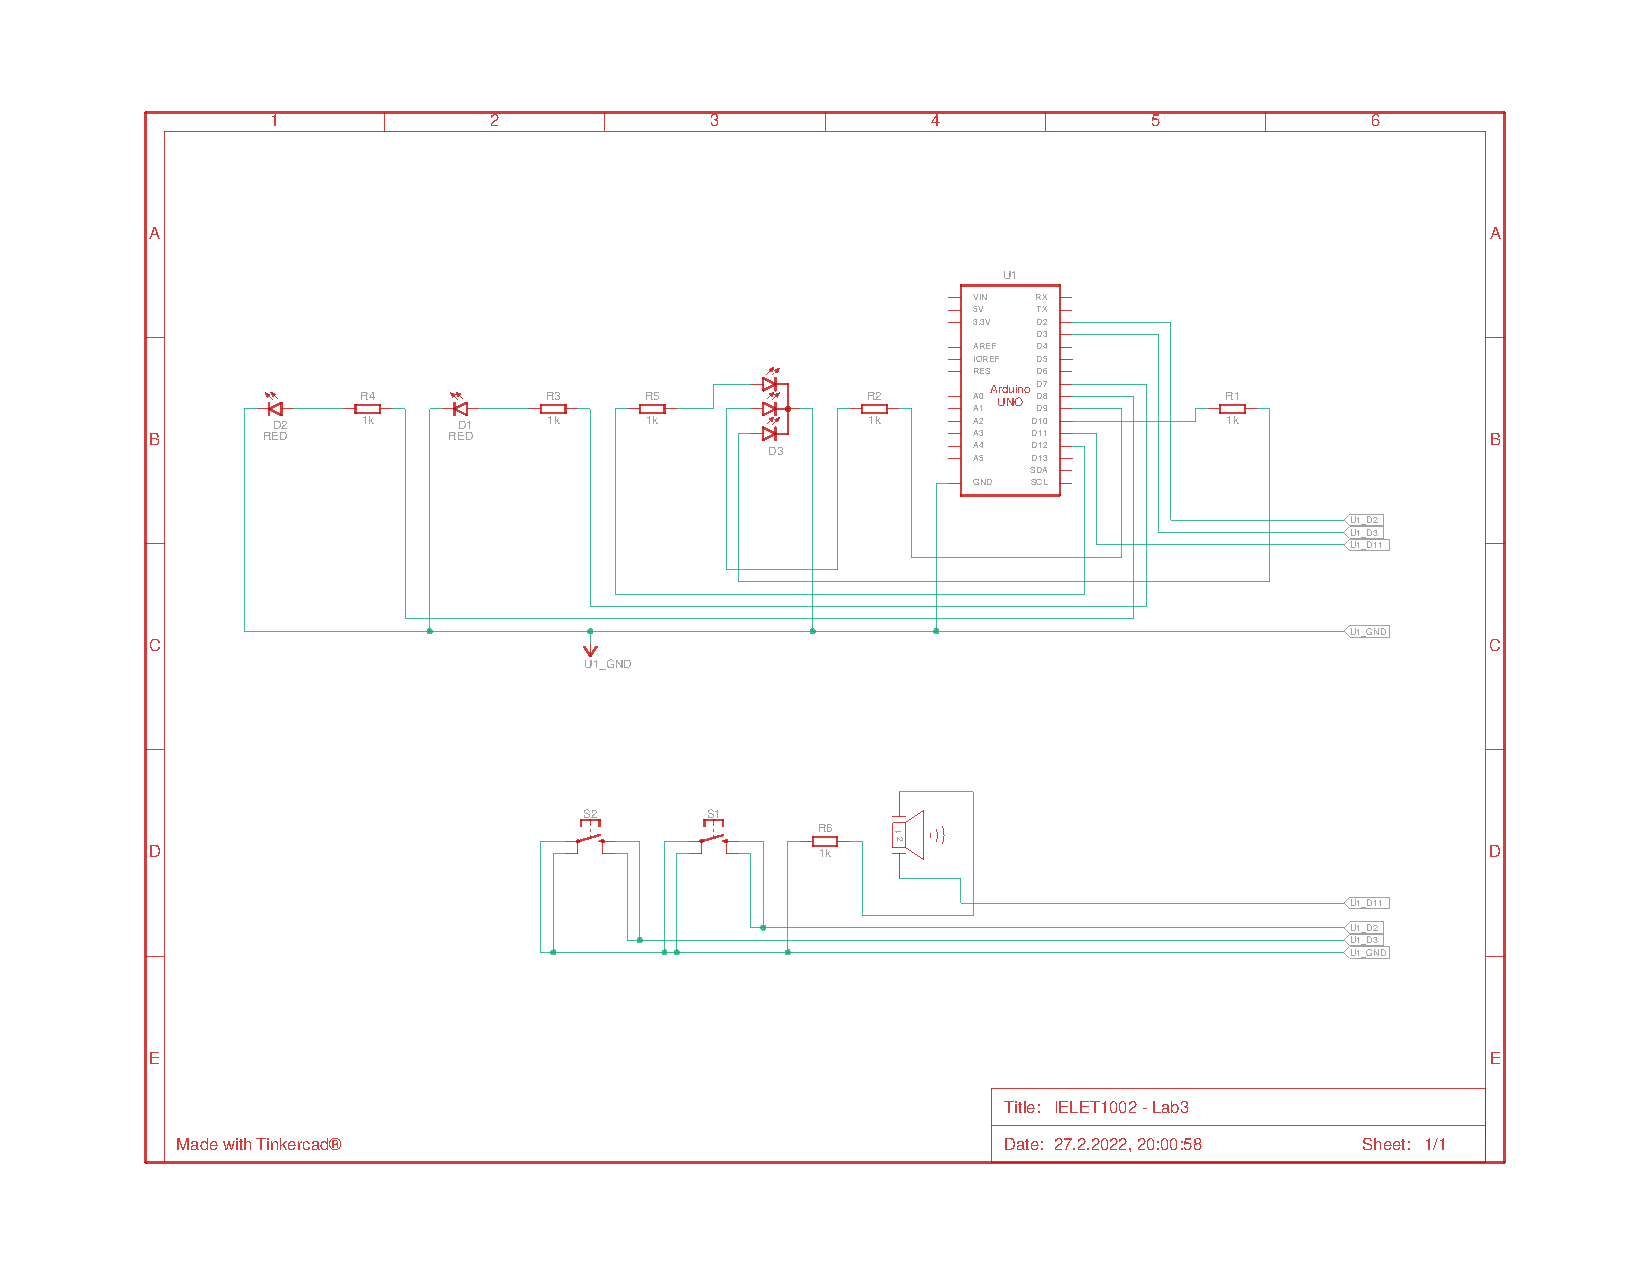
\includegraphics[width=1.5\textwidth, trim={0 2cm 0 2cm}]{images/wiring-diagram.pdf}
        \caption{Large Wiring Diagram}
        \label{fig:wiringLarge}
        \end {center}
    \end{figure}

    \begin{figure}[h]%[!ht]
        \begin {center}
        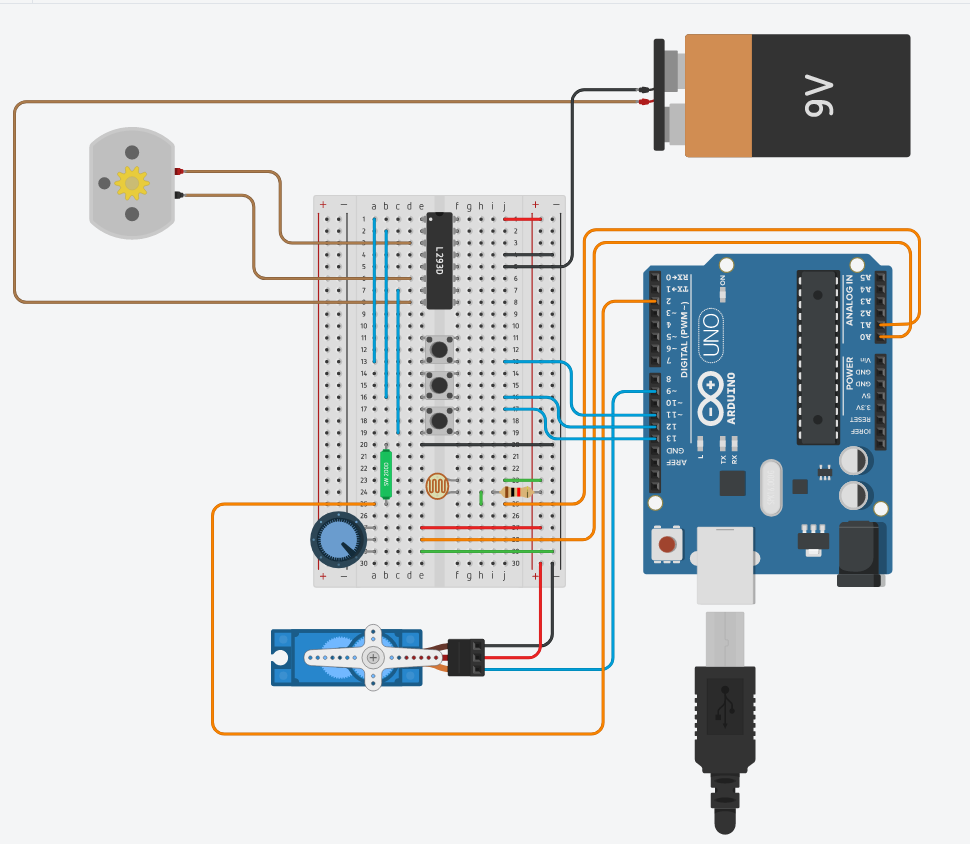
\includegraphics[width=1.2\textwidth]{images/tinkercad.PNG}
        \caption{Large Tinkercad}
        \label{fig:tinkercadLarge}
        \end {center}
    \end{figure}

\end{landscape}

\end{document}


